%% Source of figures/question-flow.pdf (rules/04-figures-tables.md).
%% Build: xelatex -output-directory=figures figures/src/question-flow.tex
%% Drawn from OpenTrading 7319264: src/core/agent.ts (runTurn), tools/wrap.ts (runTool), loop/stop-gate.ts (judgeStop).
\documentclass[border=2pt]{standalone}
\usepackage{fontspec}
\IfFontExistsTF{Arial}{\setmainfont{Arial}}{\setmainfont{TeX Gyre Heros}}
\usepackage{tikz}
\usetikzlibrary{positioning,arrows.meta,fit,backgrounds,calc}
\begin{document}
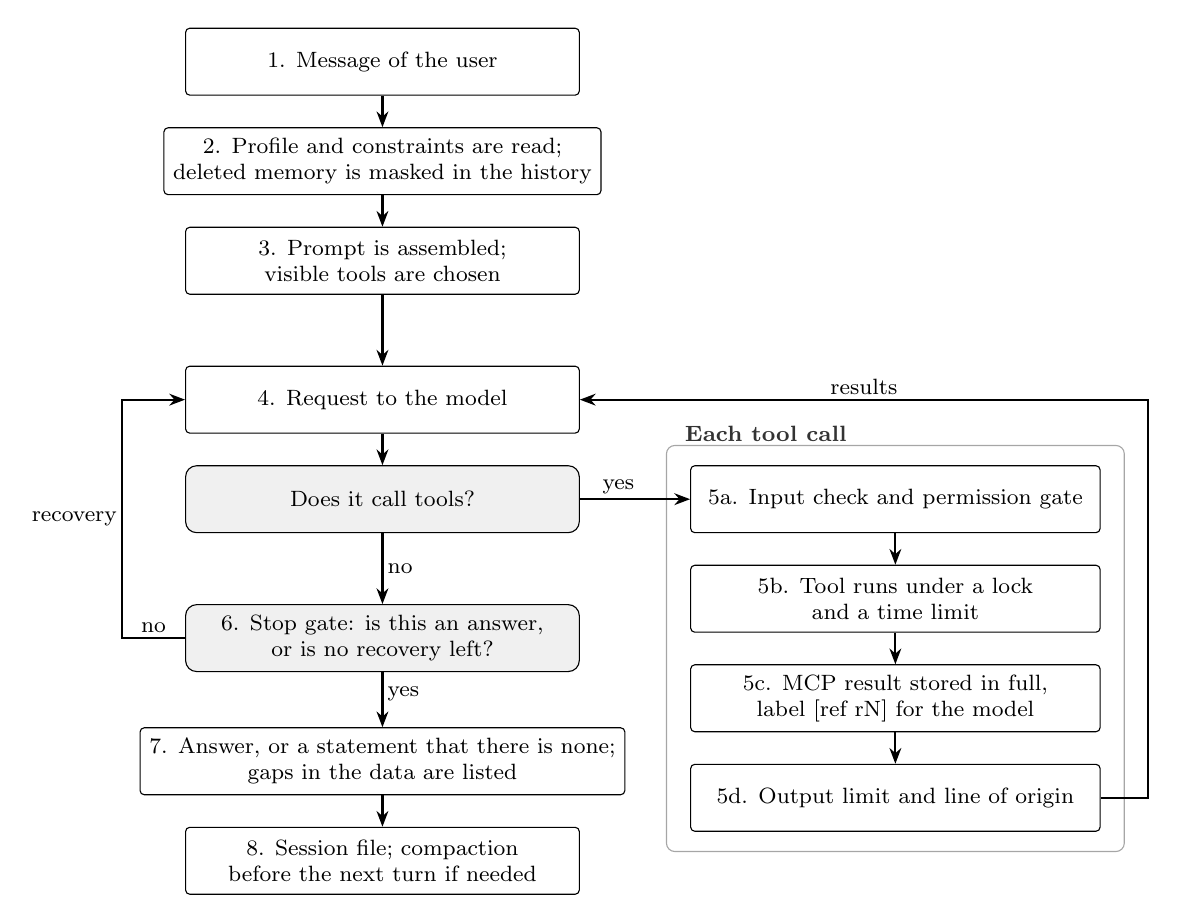
\begin{tikzpicture}[
  font=\fontsize{8}{9.5}\selectfont,
  box/.style={draw, rounded corners=1.5pt, align=center, minimum width=50mm, minimum height=8.5mm, fill=white},
  side/.style={draw, rounded corners=1.5pt, align=center, minimum width=52mm, minimum height=8.5mm, fill=white},
  dec/.style={draw, rounded corners=4pt, align=center, minimum width=50mm, minimum height=8.5mm, fill=gray!12},
  arr/.style={-{Stealth[length=2mm]}, thick},
  lab/.style={align=left, inner sep=1.5pt},
  group/.style={draw, gray!70, rounded corners=3pt, inner xsep=3mm, inner ysep=2.5mm},
  glabel/.style={font=\fontsize{8}{9.5}\selectfont\bfseries, anchor=south west, gray!40!black, inner sep=1pt}
]
\node[box] (q) {1. Message of the user};
\node[box, below=4mm of q] (bind) {2. Profile and constraints are read;\\deleted memory is masked in the history};
\node[box, below=4mm of bind] (asm) {3. Prompt is assembled;\\visible tools are chosen};
\node[box, below=9mm of asm] (ask) {4. Request to the model};
\node[dec, below=4mm of ask] (calls) {Does it call tools?};
\node[dec, below=9mm of calls] (gate) {6. Stop gate: is this an answer,\\or is no recovery left?};
\node[box, below=7mm of gate] (clean) {7. Answer, or a statement that there is none;\\gaps in the data are listed};
\node[box, below=4mm of clean] (save) {8. Session file; compaction\\before the next turn if needed};

\node[side, right=14mm of calls] (perm) {5a. Input check and permission gate};
\node[side, below=4mm of perm] (run) {5b. Tool runs under a lock\\and a time limit};
\node[side, below=4mm of run] (ref) {5c. MCP result stored in full,\\label [ref rN] for the model};
\node[side, below=4mm of ref] (cap) {5d. Output limit and line of origin};

\draw[arr] (q) -- (bind);
\draw[arr] (bind) -- (asm);
\draw[arr] (asm) -- (ask);
\draw[arr] (ask) -- (calls);
\draw[arr] (calls) -- node[lab, right] {no} (gate);
\draw[arr] (gate) -- node[lab, right, pos=0.4] {yes} (clean);
\draw[arr] (clean) -- (save);
\draw[arr] (calls.east) -- node[lab, above, pos=0.35] {yes} (perm.west);
\draw[arr] (perm) -- (run);
\draw[arr] (run) -- (ref);
\draw[arr] (ref) -- (cap);
\draw[arr] (cap.east) -- ++(6mm,0) |- node[lab, above, pos=0.75] {results} (ask.east);
\draw[arr] (gate.west) -- node[lab, above] {no} ++(-8mm,0) |- node[lab, pos=0.25, left] {recovery} (ask.west);
\begin{scope}[on background layer]
  \node[group, fit=(perm)(cap)] (tg) {};
  \node[glabel] at ([xshift=2mm]tg.north west) {Each tool call};
\end{scope}
\end{tikzpicture}
\end{document}
